\section{Outils généraux}

\subsection{Utilité de regrouper ces résultats}
Pour calculer le groupe fondamental du tore, de $\mathbb{R}$P$^2$ et de la bouteille de Klein, on utilise le théorème de Van Kampen, chaque fois appliqué à des carrés dont on identifie les bords par une relation d'équivalence.\medskip\\
Naturellement, certains schémas de preuves se répètent, et il est alors plus intéressant de regrouper les propositions principales dont on utilisera les résultats dans les calculs de ces 3 groupes fondamentaux.
Essentiellement, on séparera toujours le carré en $2$ ouverts, l'un, $U_0$, étant logé dans l'intérieur du carré, et l'autre, $V_0$, couvrant les bords. On va alors prouver que par passage au quotient, on a toujours $\tilde{U_0}$ simplement connexe, $\tilde{U_0}\cap\tilde{V_0}=\widetilde{U_0\cap V_0}$ de groupe fondamental isomorphe à $\mathbb{Z}$ et (sauf $\mathbb{R}$P$^2$ pour celui-ci) $\pi_1(V)\cong S^1\vee S^1$.

\subsection{Résultats}
Notons d'abord que pour les $3$ espaces étudiés, on se ramène chaque fois à un espace $[0,1]^2/\mathcal{R}$ avec $\mathcal{R}$ une relation d'équivalence laissant invariants les points de $]0,1[^2$. On notera aussi $I=[0,1]$.
\begin{proposition}
    Soit un ouvert $U$ de $[0,1]^2$ à valeurs dans $]0,1[^2$ (ne contenant aucun point du bord), alors il est saturé et la restriction $q_{|U}$ de l'application quotient $q:[0,1]^2\rightarrow[0,1]^2/\mathcal{R}$ est un homéomorphisme de $U$ sur son image $q(U)=\tilde{U}$
\end{proposition}
\begin{proof}
    Commençons par montrer qu'il est saturé : on a $q^{-1}(q(U))=\{p\in I^2, [p]\in q(U)\}$. Or, $U$ ne contenant aucun point du bord, l'image de chaque point par l'application quotient est la classe de cet unique point, et donc on a $p\in U\Rightarrow(x\neq p\Rightarrow p\not\sim x)$, d'où $q^{-1}([p])=\{p\}$. Il vient alors $q^{-1}(q(U))=U$.\medskip\\
    L'application $q_{|U}:U\rightarrow\tilde{U}$ est continue et surjective. Il suffit de montrer qu'elle est ouverte et injective pour qu'elle soit un homéomorphisme.\medskip\\
    \textit{Injectivité} : Soient $p,s\in U$ tels que $q_{|U}(p)=q_{|U}(s)$, donc $[p]=[s]$. Or, ces points sont dans $]0,1[^2$ donc $p\sim x\iff x=p$ pour tout $x\in[0,1]^2$, d'où $s=p$.\medskip\\
    \textit{L'application est ouverte} : soit $W$ un ouvert de $U$, alors $q_{|U}(W)=\{[p],p\in W\}$ et $q_{|U}^{-1}(q_{|U}(W))=\{p\in U,[p]\in q_{|U}(W)\}$ car $U$ est saturé et $W\subset U$. Or, par injectivité, il n'existe pas de $p\not\in W$ tel que $[p]\in q_{|U}(W)$. Il vient alors $q_{|U}^{-1}(q_{|U}(W))=W$ ouvert, et par définition de la topologie quotient $q_{|U}(W)$ est ouvert.\medskip\\
    Finalement, $q_{|U}$ est une bijection bicontinue, c'est donc un homéomorphisme.
\end{proof}
\begin{proposition}
    Le passage au quotient d'une rétraction par déformation fixant $\partial I^2$ point par point est encore une rétraction par déformation, fixant $q(\partial I^2)$ point par point.
\end{proposition}
\begin{proof}
    Soit $A$ un ouvert de $I^2$ et soit $r:I\times A\rightarrow A$ une rétraction par déformation telle que $r(0,s)=s$, $r(1,s)\in\partial I^2$ pour $s\in A$ et $r(t,s)=s$ pour $s\in\partial I^2$ et $t\in[0,1]$.
    Notons $\tilde{r}:I\times\tilde{A}\rightarrow\tilde{A}$ l'application $\tilde{r}(t,q(s))=q(r(t,s))$. Montrons qu'elle est bien définie : pour $p\sim s$, s'ils ne sont pas sur le bord, on a $p=s$ et $\tilde{r}$ est bien définie sur $q(p)$. Si $p\sim s$ et ils sont sur le bord, alors $\tilde{r}(t,q(s))=q(r(t,s))=q(s)=q(p)=q(r(t,p))=\tilde{r}(t,q(p))$ donc $\tilde{r}$ est bien définie.\medskip\\
    Il s'agit alors de montrer que $\tilde{r}$ est continue, vrai car $Id_{I}\times q$ est quotient par compacité de $I$ (la preuve de ce résultat n'est pas immédiate, et n'est pas d'un grand intérêt pour ce projet. Pour le lecteur curieux, une preuve plus générale est disponible dans le livre d'Engelking, General Topology, Thm 3.3.17), donc $\tilde{r}$ est continue si et seulement si $\tilde{r}\circ(Id_{I}\times q)=q\circ r$ est continue, ce qui est vrai car $q\circ r$ est composée d'applications continues.\medskip\\
    Enfin, $\tilde{r}$ est bien une rétraction par déformation :\\ 
    $\tilde{r}(0,q(s))=q(r(0,s))=q(s)$\\
    $\tilde{r}(1,q(s))=q(r(1,s))\in q(\partial I^2)$\\
    $q(s)\in q(\partial I^2)\iff s\in\partial I^2$ et donc $r(t,q(s))=q(r(t,s))=q(s)$, ce qui conclut.
\end{proof}
\newpage
Il est maintenant temps de s'intéresser aux ouverts $U_0$ et $V_0$ précis que l'on utilisera dans chaque calcul. On a alors $U_0=]\frac{1}{4},\frac{3}{4}[^2$ et $V_0=\left([0,\frac{3}{8}[\cup]\frac{5}{8},1]\right)\times[0,1]\cup[0,1]\times\left([0,\frac{3}{8}[\cup]\frac{5}{8},1]\right)$. Dessins ci-dessous\medskip\\
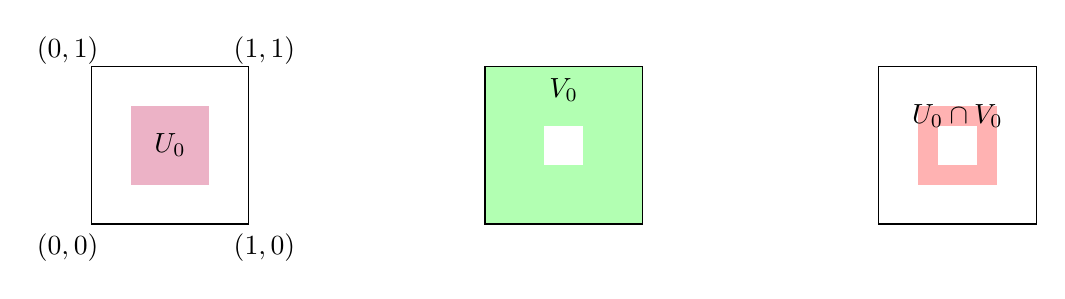
\begin{tikzpicture}
    \fill[purple!30] (0.5, 0.5) rectangle (1.5, 1.5);
    \draw (0,0) rectangle (2,2);
    \node at (1, 1) {$U_0$};
    \foreach \x in {0,1} {
    \foreach \y in {0,1} {
        \node at (\x*2.5-0.3,\y*2.5-0.3) {$(\x,\y)$};
    }
    }
    \begin{scope}[xshift=5cm]
        \fill[green!30] (0,0) rectangle (2,2);
        \fill[white] (3/4, 3/4) rectangle (5/4, 5/4);
        \draw (0,0) rectangle (2,2);
        \node at (1, 1.7) {$V_0$};
    \begin{scope}[xshift=5cm]
    \fill[red!30] (0.5,0.5) rectangle (1.5,1.5);
        \fill[white] (3/4, 3/4) rectangle (5/4, 5/4);
        \draw (0,0) rectangle (2,2);
        \node at (1, 1.37) {$U_0\cap V_0$};
    \end{scope}
    \end{scope}
\end{tikzpicture}
\bigskip\\
Le passage au quotient induit deux ouverts $\tilde{U}_0$ et $\tilde{V}_0$. Notons que $U_0$ et $V_0$ sont saturés par passage au quotient ($U_0$ est inclus dans l'intérieur et $V_0$ contient simultanément tous les points de la frontière).
\begin{corollaire}
    $U_0$ est homéomorphe à $\tilde{U}_0$ et est simplement connexe
\end{corollaire}
\begin{proof}
    $U_0$ n'admettant aucun élément de $\partial I^2$, l'homéomorphisme se déduit directement de la \textbf{Proposition 2.1}. Il suffit alors de montrer qu'il est simplement connexe, ce qui est trivial car il est convexe. Une rétraction par déformation de $U_0$ sur $c=(\frac{1}{2},\frac{1}{2})$ est $r:I\times U_0\rightarrow U_0$, $r(t,s)=(1-t)s+tc$. On a donc $\pi_1(\tilde{U}_0)\cong\pi_1(U_0)\cong*$ où $*$ est le groupe trivial.
\end{proof}
\begin{proposition}
    On a $\tilde{U}_0\cap\tilde{V}_0=\widetilde{U_0\cap V_0}$ et $\pi_1(\tilde{U}_0\cap\tilde{V}_0)\cong\mathbb{Z}$.
\end{proposition}
\begin{proof}
    \textit{$\tilde{U}_0\cap\tilde{V}_0=\widetilde{U_0\cap V_0}$} : Si $[p]\in\tilde{U}_0\cap\tilde{V}_0$ alors $[p]\in\tilde{U}_0$ donc c'est la classe de l'unique élément $p$, qui appartient à la fois à $U_0$ et $V_0$. On a donc $[p]\in\widetilde{U_0\cap V_0}$. D'autre part, l'inclusion $\widetilde{U_0\cap V_0}\subset\tilde{U}_0\cap\tilde{V}_0$ est immédiate.\medskip\\
    \textit{$\pi_1(\tilde{U}_0\cap\tilde{V}_0)\cong\mathbb{Z}$} : On va définir une rétraction par déformation de $U_0\cap V_0$ sur un carré, homéomorphe à $S^1$.\\
    On a d'abord $U_0\cap V_0=\left(]\frac{1}{4},\frac{3}{8}[\cup]\frac{5}{8},\frac{3}{4}[\right)\times]\frac{1}{4},\frac{3}{4}[\cup]\frac{1}{4},\frac{3}{4}[\times\left(]\frac{1}{4},\frac{3}{8}[\cup]\frac{5}{8},\frac{3}{4}[\right)$\medskip\\
    Visuellement, il parait raisonnable de déformer cette aire en un carré centré en son intérieur, et c'est précisément ce que l'on va faire, en utilisant pour tout point $s$ de $U_0\cap V_0$, l'intersection entre le segment qui le relie à $c$ et le carré vers lequel on va se rétracter. En étudiant les bords $(\frac{5}{8},\frac{5}{8})$ et $(\frac{3}{4},\frac{3}{4})$, on trouve comme milieu $(\frac{11}{16},\frac{11}{16})$. On veut alors paramétriser le carré passant par ce point et de centre $c=(\frac{1}{2},\frac{1}{2})$, du moins avoir une relation d'un point de l'aire au point $\pi(s)$ du carré vers lequel on va le rétracter. Ainsi, la distance en norme infinie de ce carré au centre est égale à $||(\frac{11}{16},\frac{11}{16})-c||_{\infty}=\frac{3}{16}$. On peut alors aisément définir la rétraction par déformation, car ici on aura $\pi(s)=\lambda s+(1-\lambda)c$ avec $\lambda\in]0,1[$ car dans le segment $[c,s]$ et $\frac{3}{16}=||\pi(s)-c||_{\infty}=||\lambda(s-c)||_{\infty}$ d'où $\lambda=\frac{3}{16||s-c||_{\infty}}$, soit $\pi(s)=c+\displaystyle\frac{3(s-c)}{16||s-c||_{\infty}}$, valide car $s\neq c$ car $c\not\in U_0\cap V_0$.
    
    On définit alors une rétraction par déformation \\
    $r:I\times U_0\cap V_0\rightarrow U_0\cap V_0$ par $r(t,s)=t\pi(s)+(1-t)s=t\left(c+\displaystyle\frac{3(s-c)}{16||s-c||_{\infty}}\right)+(1-t)s$.\medskip\\
    Le passage au quotient induit un homéomorphisme $q_{|U_0\cap V_0}:U_0\cap V_0\rightarrow\tilde{U}_0\cap\tilde{V}_0$ (car $\widetilde{U_0\cap V_0}=\tilde{U}_0\cap\tilde{V}_0$) par la \textbf{Proposition 2.1.}, car $U_0\cap V_0$ ne touche pas le bord, et il ne reste plus qu'à montrer que le carré des $\pi(s)$ est homéomorphe à $S^1$. Montrons le pour le carré $\partial I^2$, le résultat cherché étant direct par transformation affine.\medskip\\
    Soit $f:\partial I^2\rightarrow S^1$ définie par $f(t,0)=e^{\frac{i\pi}{2}t},f(1,t)=e^{\frac{i\pi}{2}(t+1)},f(t,1)=e^{\frac{i\pi}{2}(3-t)},f(0,t)=e^{\frac{i\pi}{2}(4-t)}$. Essentiellement, on fait le tour du cercle quart par quart selon le côté du carré où l'on est. Cette fonction est continue, injective et surjective donc bijective et bicontinue car sur un compact, c'est bien un homéomorphisme de $\partial I^2$ sur $S^1$. La transformation affine $j(\pi(s))=\frac{8}{3}(\pi(s)-c)+c$ est un homéomorphisme nous donnant $f\circ j$ l'homéomorphisme entre le carré des $\pi(s)$ et $S^1$.\newpage
    Finalement, puisque $q_{|U\cap V}$ est un homéomorphisme, l'image du carré dans $\tilde{U}_0\cap\tilde{V}_0$ est homéomorphe à ce même carré, lui même homéomorphe à $S^1$ par $f\circ j$.\medskip\\
    On en conclut $\pi_1(\tilde{U}_0\cap\tilde{V}_0)\cong\pi_1(U_0\cap V_0)\cong\pi_1(S^1)\cong\mathbb{Z}$.
\end{proof}
Il ne reste plus qu'à traiter le cas de $V_0$. On ne va pas pouvoir raisonner par homéomorphisme ici à cause des bords, mais on va d'abord utiliser la \textbf{Proposition 2.2.} pour se donner une rétraction par déformation de $\tilde{V}_0$, puis on se donnera un résultat sur $q(\partial I^2)$ qui nous permettra de conclure. Commençons par la rétraction :
\begin{lemme}
    $V_0$ se rétracte par déformation sur $\partial I^2$ et induit une rétraction par déformation de $\tilde{V}_0$ sur $q(\partial I^2)$
\end{lemme}
\begin{proof}
    En raisonnant de la même manière (se rétracter sur un carré, ici $\partial I^2$) qu'avec la proposition précédente, on a $\pi(s)=\lambda s+(1-\lambda)c$ avec $\lambda>0$, donc $||\pi(s)-c||_{\infty}=\frac{1}{2}\iff||\lambda s+(1-\lambda)c-c||_{\infty}=\frac{1}{2}\iff\lambda=\displaystyle\frac{1}{2||s-c||_{\infty}}$.\\
    On a alors $\pi(s)=c+\displaystyle\frac{s-c}{2||s-c||_{\infty}}$
    La rétraction ainsi définie est $r:I\times V_0\rightarrow V_0$ telle que $r(t,s)=t\pi(s)+(1-t)s=t\left(c+\displaystyle\frac{s-c}{2||s-c||_{\infty}}\right)+(1-t)s$.\medskip\\
    En utilisant la \textbf{Proposition 2.2.}, il vient une rétraction $\tilde{r}:I\times\tilde{V}_0\rightarrow\tilde{V}_0$ telle que $\tilde{r}(t,q(s))=q(r(t,s))$, et elle vérifie bien le résultat attendu : $\tilde{r}(1,q(s))=q(r(1,s))=q(\pi(s))\in q(\partial I^2)$ (la stabilité de $\tilde{r}$ pour $q(\partial I^2)$ vient du fait que $\pi(s)=s$ si $s\in\partial I^2$).
\end{proof}
Il ne reste plus qu'une proposition à prouver :
\begin{proposition}
    Soit $\mathcal{R}$ une relation d'équivalence sur $\partial I^2$, vérifiant :\\
    - $(t,0)\sim(t,1), t\in[0,1]$ ou $(t,0)\sim(1-t,1),t\in[0,1]$\\
    et\\
    - $(0,t)\sim(1,t),t\in[0,1]$ ou $(0,t)\sim(1,1-t),t\in[0,1]$\\
    (donc on identifie les points de côtés opposés soit dans le même sens, soit en sens inverse), et identifiant les $4$ coins du carré en une seule classe. Alors $q(\partial I^2)\cong S^1\vee S^1$
\end{proposition}
\begin{proof}
    On a d'abord $S^1\vee S^1\cong S^1\times\{1\}\cup\{1\}\times S^1$, qu'on manipulera par souci de simplicité.\\
    Soit $f:q(\partial I^2)\rightarrow S^1\times\{1\}\cup\{1\}\times S^1$, définie par $f([(t,0)])=(e^{2i\pi t},1)$ et $f([(1,t)])=(1,e^{2i\pi t})$. $f$ est continue car $f\circ q=\overline{f}:\partial I^2\rightarrow S^1\times\{1\}\cup\{1\}\times S^1$ est continue :\medskip\\
    Sur $(t,0)$ et $(1,t)$, c'est évident. Montrons que pour leurs côtés opposés, $\overline{f}$ est aussi continue : on a $\overline{f}(t,1)=\overline{f}(t,0)$ ou $\overline{f}(t,1)=\overline{f}(1-t,0)$ selon la relation d'équivalence, rendant toujours $\overline{f}$ continue  sur ses côtés (de même pour $(0,t)$). La fonction est continue sur les côtés et aussi sur les coins car les côtés sont fermés. Il vient donc $\overline{f}$ continue, et $f$ aussi. De plus, $f$ est surjective par construction, et il ne reste plus qu'à montrer que $f$ est injective, car la compacité de $q(\partial I^2)$ induira la bicontinuité.\medskip\\
    \textit{Injectivité} : soient $[p]$, $[s]$ tels que $f([p])=f([s])$. Si leur image est $(1,1)$, alors $[p]=[s]$ car c'est la classe des coins. Sinon, leur image est dans le même cercle, et spdg $f([p])=(e^{2i\pi t},1)=f([s])$ donc $[p]=[(t,0)]=[s]$, encore par construction de $f$.\medskip\\
    $f$ est donc bijective et bicontinue et définit un homéomorphisme de $q(\partial I^2)$ dans $S^1\times\{1\}\cup\{1\}\times S^1$, ce qui démontre que $q(\partial I^2)\cong S^1\vee S^1$.
\end{proof}
Le cas de $\mathbb{R}$P$^2$ ne vérifie pas cette dernière proposition (car les $4$ coins du carré ne sont pas identifiés en une seule classe), et devra être traité à part. Le corollaire suivant ne vaut donc que pour les cas du tore et de la bouteille de Klein.
\begin{corollaire}
    On a $\pi_1(\tilde{V}_0)\cong\mathbb{Z}*\mathbb{Z}$
\end{corollaire}
\begin{proof}
    Par le \textbf{Lemme 2.1.} et la \textbf{Proposition 2.4.}, cela revient à démontrer que $\pi_1(S^1\vee S^1)\cong\mathbb{Z}*\mathbb{Z}$.\medskip\\
    On applique alors le théorème de Van Kampen sur les $2$ ouverts $S^1\times\alpha$ et $\alpha\times S^1$ qui recouvrent $S^1\vee S^1$, avec $\alpha=S^1\backslash\{-1\}$ par exemple. Leur intersection donne $\alpha\times\alpha$ qui se rétracte en le point $(1,1)$ donc de groupe fondamental trivial, et chaque ouvert se rétracte en $S_1\times\{1\}$ et $\{1\}\times S^1$ de groupe fondamental isomorphe à $\mathbb{Z}$. Dès lors, $\pi_1(S^1\vee S^1)\cong\mathbb{Z}*\mathbb{Z}$, ce qui conclut.
\end{proof}
